\begin{figure}
    \centering
    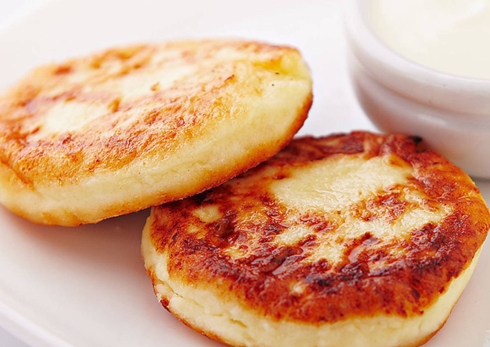
\includegraphics[width=.35\textwidth]{aleksandra/sirnik.png}
\end{figure}

\begin{recipe}
    [ % Optionale Eingaben
        preparationtime = {\unit[max. 45]{min}},
        portion = für drei Personen und es bleibt noch ein wenig übrig für Morgen,
        source = Aleksandra
    ]
    {Sirniki}

    \introduction{
        \# die beste Gesellschaft für Tee
    }


\ingredients
{% Zutatenliste
    \unit[500]{g} & Quark (möglichst trocken)\\
    \unit[1-2]{} & Eier \\
    \unit[2-4]{EL} & Zucker \\
    \unit[3-5]{EL} & Mehl \\
     & Sonnenblumen-/Rapsöl \\
    mögl. & Backpulver \\
    mögl. & Rosinen/ \\
    & Cranberries/ \\
    & Apfelstücke
}

\preparation
{ % Schrittweise Zubereitung
\\
Achtung, damit der Teig zusammenpappt und nicht auseinanderläuft muss er möglichst viel Flüssigkeit verlieren. Dafür muss er min. 24\,h abtropfen. Dazu kann er in einem Sieb oder einem Stück Mull über der Spüle aufgehangen werden. Vor der Zubereitung kann man das Paket nochmal quetschen.

Alle Zutaten in einer Schüssel miteinander verkneten, bis eine Masse entsteht, die die Konsistenz von weicher Knete oder Kartoffelpüree ähnelt.

Daraus Kreise kneten, die etwa handflächengroß und daumendick oder dicker sind. 
In der Pfanne von beiden Seiten goldbraun werden lassen. Je nach Pfanne und Hitzestufe braucht jeder Sirnik 2-5 Minuten.

Essen kann man Sirniki pur, mit Schmand, Honig oder Marmelade zu einer heißen Tasse Tee. Sie schmecken auch kalt gut.
}

\hint
{% Hinweise
Um die einzelnen Sirniki zu formen hilft es, wenn die Hand angemehlt ist. Dann erst Kugeln formen und sie anschließend zerdrücken.\\ 
Am schnellsten (aber auch stressigsten) geht es, die Pfanne zu erhitzen, bis das Öl heiß wird, die ersten Sirniki vorzubereiten und braten, sobald das Öl heiß ist. Während sie brutzeln, kann man dann die nächsten vorbereiten. \\
Viel Öl hilft viel. \\
Einen Teller bereithalten, um die fertigen Sirniki abzulegen. Um das Pfannenfett einzusaugen, kann man auf den Teller ein Papiertuch legen.        
}

    \end{recipe}
